\documentclass[12pt, letterpaper]{article}
\usepackage{graphicx}
\usepackage[margin=3cm]{geometry}
\usepackage{float}
\usepackage{hyperref}
\usepackage[style=mla, backend=biber]{biblatex}
\graphicspath{{/Users/teddy/Developer/Latex/images}}
\renewcommand{\familydefault}{\sfdefault}
\newcommand{\var}[1]{
   \textit{#1}
}

\addbibresource{ipp_os.bib} 

\title{
Writing My Own Operating System In Rust\\
\large An Expolration Into Computer Archetecture
}
\author{Teddy Maloney}
\date{June 5, 2023}
\begin{document}

\maketitle

\section{What is an Operating System Kernel?}

An operating system kernel is the central component of an operating system that serves as a core bridge between 
software applications and the underlying hardware of a computer system. It manages system resources, provides 
essential services, and facilitates communication between software and hardware.

The kernel manages various aspects of the system, including process management, memory management, 
and input/output operations. It schedules and coordinates the execution of processes, ensuring fair allocation 
of CPU time and efficient multitasking. Additionally, it manages memory by allocating and deallocating memory 
to processes, optimizing memory usage, and providing memory protection.

The kernel also handles input/output operations, allowing software applications to interact with peripheral 
devices such as disks, printers, and networks. It provides device drivers as translators between the hardware 
and the software, enabling communication and data transfer.

\newpage

\section{What Can My Kernel Do?}

\subsection{Memory Paging}
My OS kernel uses page tables to convert virtual memory addresses to physical memory addresses. 
The page tables serve as a maps between the two address spaces. When a program accesses virtual memory, 
the kernel consults the page tables for the corresponding physical address. If a valid mapping exists, 
the operation is directed to the correct physical location. If not, a process called page fault 
handling is triggered. This involves retrieving data from secondary storage and allocating new physical 
memory. The page table is updated with the new mapping, enabling future accesses to be translated directly 
to the physical memory location. This mechanism allows efficient memory management and supports 
multitasking across different processes.

\begin{figure} [H]
      \centering
      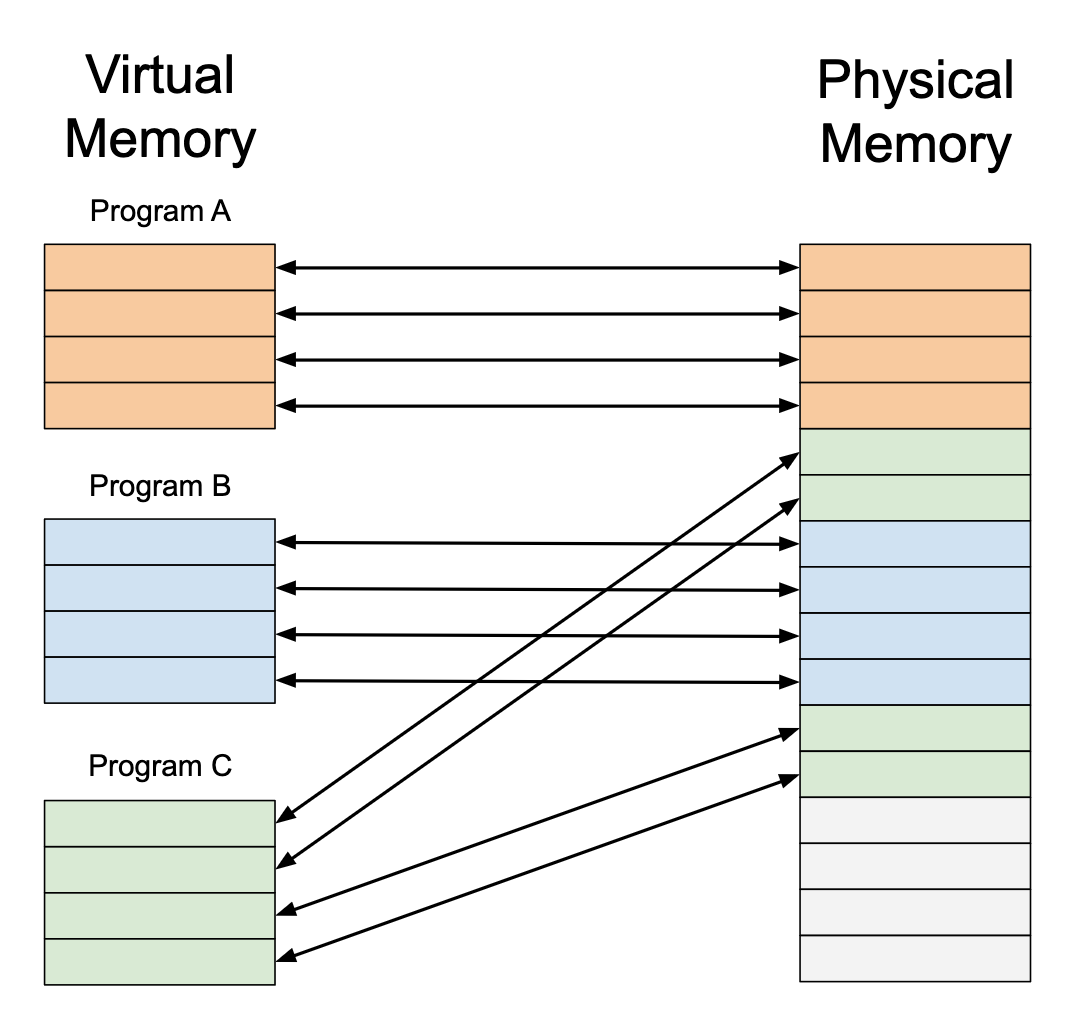
\includegraphics[width=0.75\textwidth]{paging.png}
      \caption{Translating virtual adresses to physical adresses}
      \label{fig:paging}
\end{figure}

\newpage

\subsection{Printing To The VGA Buffer}
A VGA (Video Graphics Array) buffer, also known as a frame buffer, is a region of memory in a computer's graphics 
system that stores the pixel data necessary to generate images on a display. It acts as an intermediary between the 
computer's software and the physical display hardware, allowing for efficient rendering and manipulation of graphical 
content.

To write to a VGA buffer, the software interacts with the memory addresses reserved for the frame buffer. Each 
memory location within the buffer corresponds to a pixel on the display. By modifying the pixel values stored in 
the buffer, the software can control the appearance and arrangement of visual elements on the screen.

\begin{figure}[H]
      \centering
      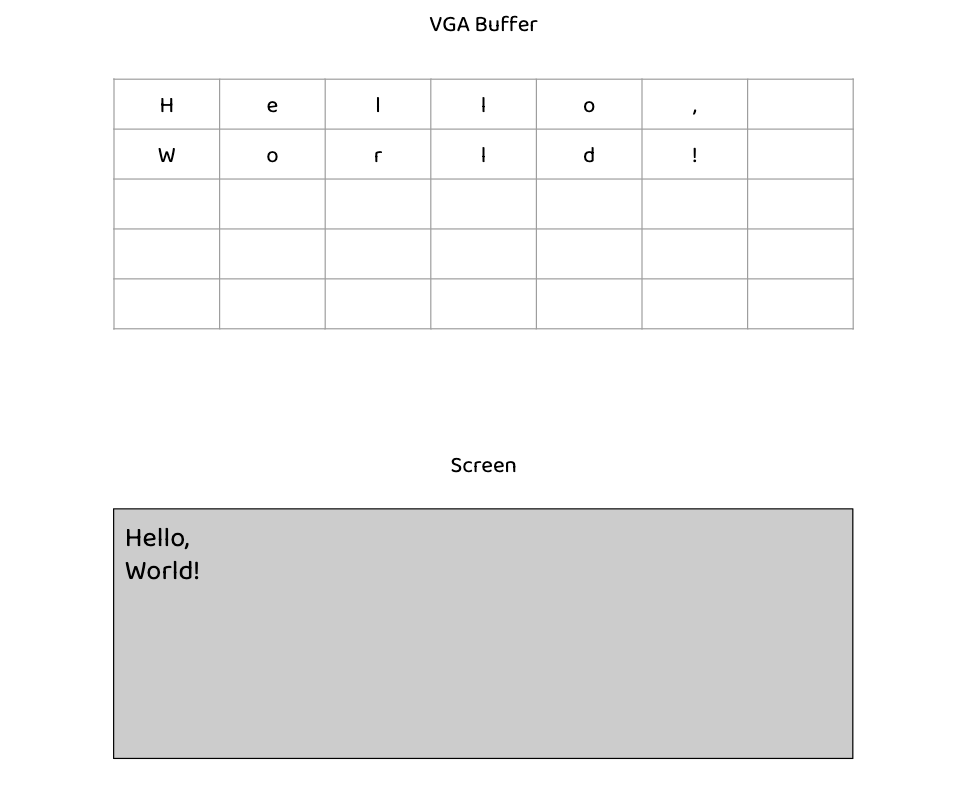
\includegraphics[width=0.75\textwidth]{vga_buffer.png}
      \caption{A comparison of the VGA buffer to a screen}
      \label{fig:vga_buffer}
\end{figure}

We can also take peripheral inputs and print them to the screen using interrupts.

\subsection{Interrups And Taking Keyboard Inputs}

Interrupts are essential mechanisms in computer systems that handle immediate events, like keyboard inputs. 
When a key is pressed, the keyboard controller triggers a hardware interrupt to notify the CPU. The CPU pauses 
its current task and executes an interrupt handler specifically designed for keyboard input. The handler 
captures the keystrokes and prints them to the VGA buffer. The CPU then resumes its previous task or switches 
to another task. Interrupts enable efficient and timely management of keyboard inputs in computer systems.

\subsection{Memory Management}

My kernel manages dynamic memory by using a simple linked list allocator. For more information read the How Does 
My Kernel Manage Memory section.

\section{What is Hardware and Software?}

\subsection{Hardware}
Hardware refers to the physical components of a computer system, such as the motherboard, CPU, memory modules, 
storage devices, input/output devices, and peripherals. It encompasses the tangible, electronic, and mechanical 
parts that form the foundation of a computer system. Hardware components are responsible for executing instructions 
and performing calculations. They provide the necessary interfaces for communication with other hardware, firmware, 
and software components.

\subsection{Firmware}
Firmware sits between hardware and software. It is a type of software that is embedded into hardware devices or 
components during the manufacturing process. Firmware provides low-level control and instructions specific to the 
hardware it is installed on. It is typically stored in non-volatile memory, such as ROM (read-only memory) or 
flash memory which doesn't need constant power to be stored. Firmware controls hardware devices' basic 
functionalities and initialization processes, enabling them to work seamlessly with the rest of the computer 
system. Examples of firmware include the BIOS (\textbf{B}asic \textbf{I}nput/\textbf{O}utput \textbf{S}ystem) in a computer.

\subsection{Software}
Software refers to the programs, data, and instructions that run on a computer system. It is a collection of 
codes and algorithms written in programming languages that provide specific functionalities and services to 
users. Software can be classified into system software (such as operating systems and device drivers) that 
manages and controls the hardware resources and application software (such as word processors, web browsers, 
and games) that are designed for specific tasks or user requirements. Software is typically stored in non-volatile 
storage devices such as hard drives or solid-state drives and is loaded into the computer's memory for execution.

\newpage

\section{Integral Hardware Components}
\begin{itemize}
      \item \textbf{Central Processing Unit (CPU)}: The CPU is the "brain" of the computer that executes instructions, performs calculations, and manages data processing. It consists of the arithmetic logic unit (ALU), control unit, registers, and cache.

      \begin{itemize}
	      \item \textbf{Arithmetic Logic Unit (ALU)}: The ALU is responsible for performing arithmetic (such as addition, subtraction, multiplication, and division) and logical operations (such as AND, OR, and NOT) on data. It carries out calculations and comparisons for processing instructions and manipulating data within the CPU.
	
	      \item \textbf{Control Unit (CU)}: The Control Unit manages the execution of instructions within the CPU. It fetches instructions from memory, decodes them, and controls the flow of data between different CPU components. The Control Unit also coordinates the timing and sequencing of instructions, ensuring that they are executed in the correct order.
	
	      \item \textbf{Registers}: Registers are small, high-speed memory units located within the CPU. They store data and instructions that are currently being processed by the CPU. Registers provide quick access to data, allowing for faster execution of instructions. Common types of registers include the program counter (PC), which holds the memory address of the next instruction to be fetched, and general-purpose registers (like the accumulator) used for various calculations and data manipulation.
      
            \begin{figure}[H]
                  \centering
                  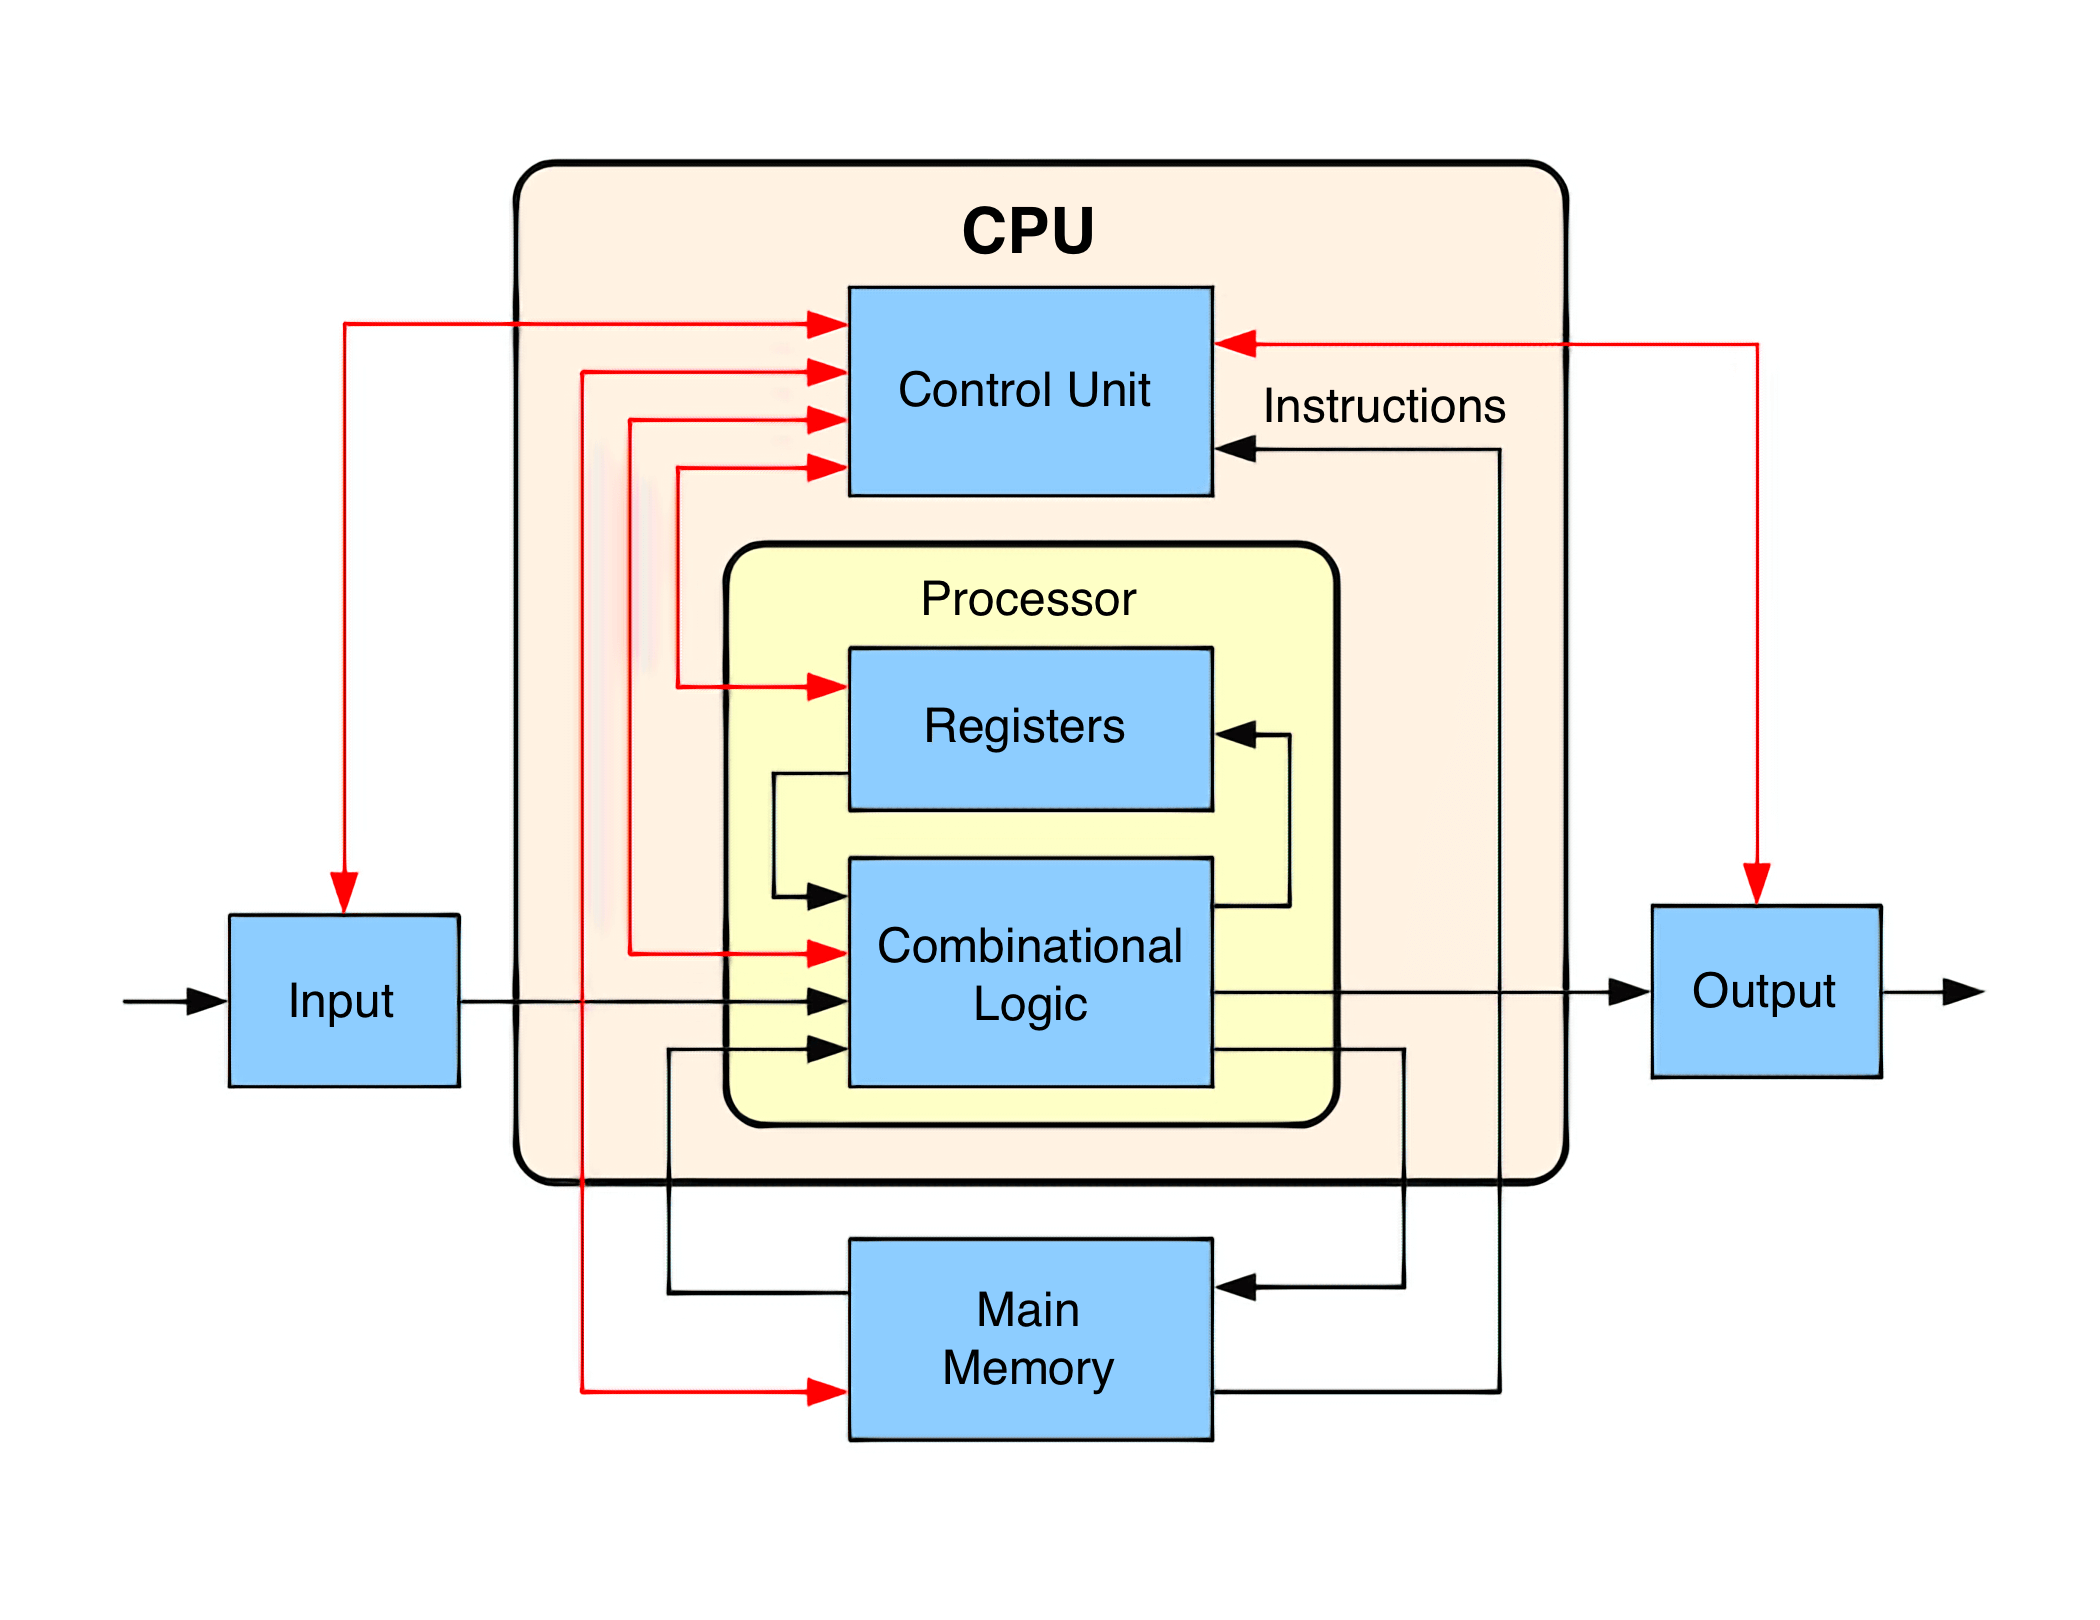
\includegraphics[width=0.75\textwidth]{cpu.png}
                  \caption{A diagram of the CPU}
                  \label{fig:cpu}
            \end{figure}
            \cite{image1}

      \end{itemize}

      \item \textbf{Random Access Memory (RAM)}: RAM is the primary memory of a computer system that stores data and instructions temporarily while the CPU is actively using them. It provides fast access to data, allowing for quick read and write operations.

      \item \textbf{Motherboard}: The motherboard is the main circuit board of a computer system. It connects and houses various components, including the CPU, memory modules, expansion cards, and other essential peripheral
\end{itemize}

\section{What is Memory?}

Memory(RAM) stores data, instructions, and program code for current or future use by the CPU (Central Processing Unit). It is a crucial part of a computer's architecture and plays a vital role in the overall performance and functionality of a system. There are two different ways memory is stored on your computer.

\begin{enumerate}
      \item Stack: The stack is a region of memory used for storing local variables and function call information. It is managed by the CPU and operates in a Last-In, First-Out (LIFO) manner. When a function is called, its local variables and return address are pushed onto the stack, creating a new stack frame. As functions complete, their stack frames are removed from the top of the stack. The stack is typically faster to access and has a fixed size determined during program compilation.
      \item Heap: The heap is a region of memory used for dynamic memory allocation. It is a pool of memory where objects and data can be allocated and deallocated as needed. Unlike the stack, memory allocation in the heap is not always managed automatically. Developers sometimes explicitly request memory from the heap using functions like `alloc()` and are responsible for freeing it when no longer needed using `dealloc()`.  Some languages, like java, have a built in heap manager called garbage collection that will automatically free memory when it is no longer needed. The heap provides greater flexibility in memory management but can be slower to access and requires manual memory management to avoid memory leaks and fragmentation.
\end{enumerate}

\begin{figure}[H]
      \centering
      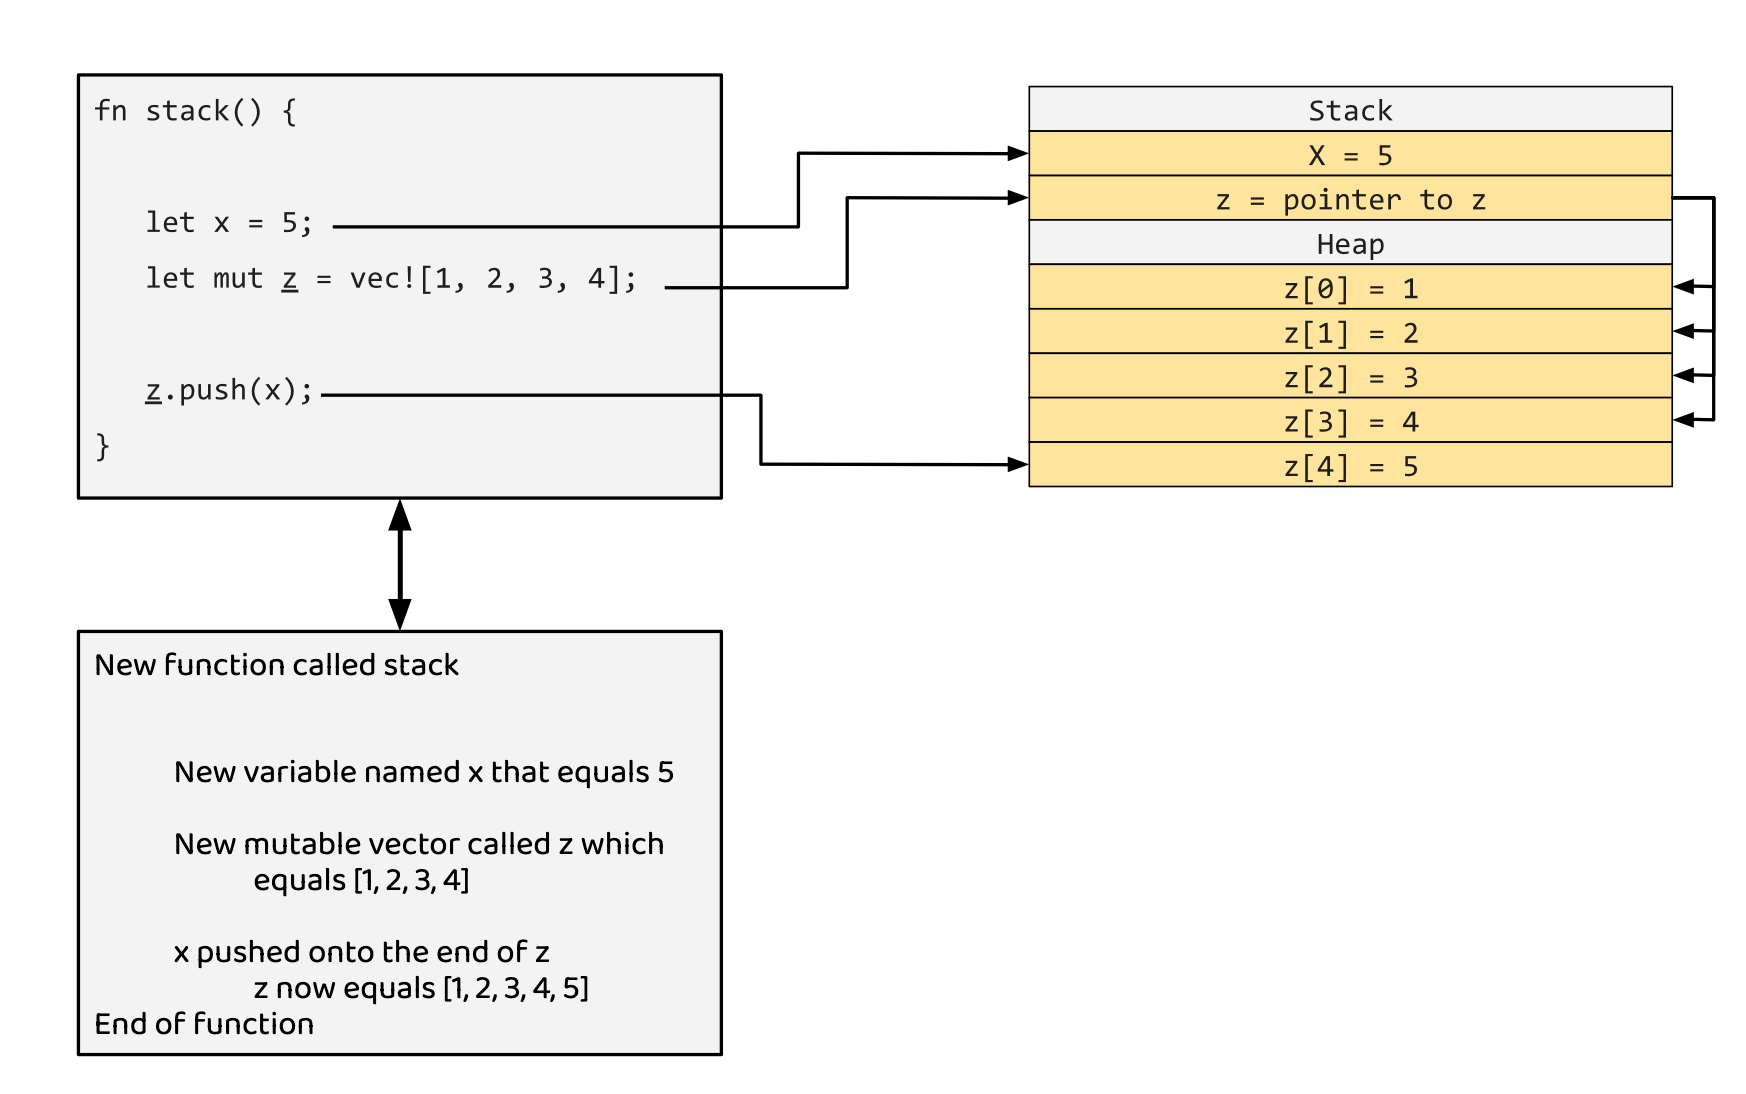
\includegraphics[width=0.75\textwidth]{stack.png}
      \caption{A Diagram of the stack and heap}
      \label{fig:stack}
\end{figure}

\begin{Large} \center \noindent This previous code can be explained by the following sequence: \end{Large}

\bigskip


\noindent \textbf{Function Entry}:
When the stack() function is called, the function's stack frame is created.
The stack frame includes space for storing local variables, function arguments, return addresses, and other bookkeeping information.
The stack frame is typically limited in size and is managed automatically by the program's execution environment.

\medskip

\noindent \textbf{Stack Variables}:
Inside the stack() function, two variables are declared: x and z.
The x variable is a simple i32 type and will be allocated on the stack. It will consume a fixed amount of memory to store the value 5.

\medskip

\noindent \textbf{Vector z}:
The z variable is a Vec<i32> type, which is a dynamically sized container. It will allocate memory on both the stack and the heap.
On the stack, the Vec struct itself will be stored, which contains metadata about the vector, such as its length and capacity.
On the heap, the actual elements of the vector will be stored. In this case, it will initially contain [1, 2, 3, 4].

\medskip

\noindent \textbf{Push Operation}:
The z.push(x) operation will add the value of x (which is 5) to the end of the vector.
If the vector's capacity is not sufficient to hold the new element, it will trigger a reallocation on the heap to allocate additional memory.
The existing elements of the vector will be copied to the newly allocated memory, and the new element (5) will be added at the end.

\medskip

\noindent \textbf{Function Exit}:
When the stack() function finishes executing, the stack frame will be deallocated, and the memory associated with local variables (x and z) will be freed.
The vector z will deallocate its heap memory automatically, as it follows Rust's ownership and borrowing rules.

\section{How Does My Kernel Manage Memory?}

Dynamic memory is allocated at runtime for storing data. An allocator manages by tracking available space, and 
allocating memory blocks. It allows programs to handle varying data requirements and create dynamic data structures.

\subsection{Bump Allocator:}

The bump allocator is an efficient method for managing memory. It works by creating a pointer called \var{next}, 
which points to the beginning of unused memory. When a new block of memory is needed, the allocator moves \var{next} 
to the new beginning of the unused memory as seen in Figure \ref{fig:mem1}.

\begin{figure}[H]
      \centering
      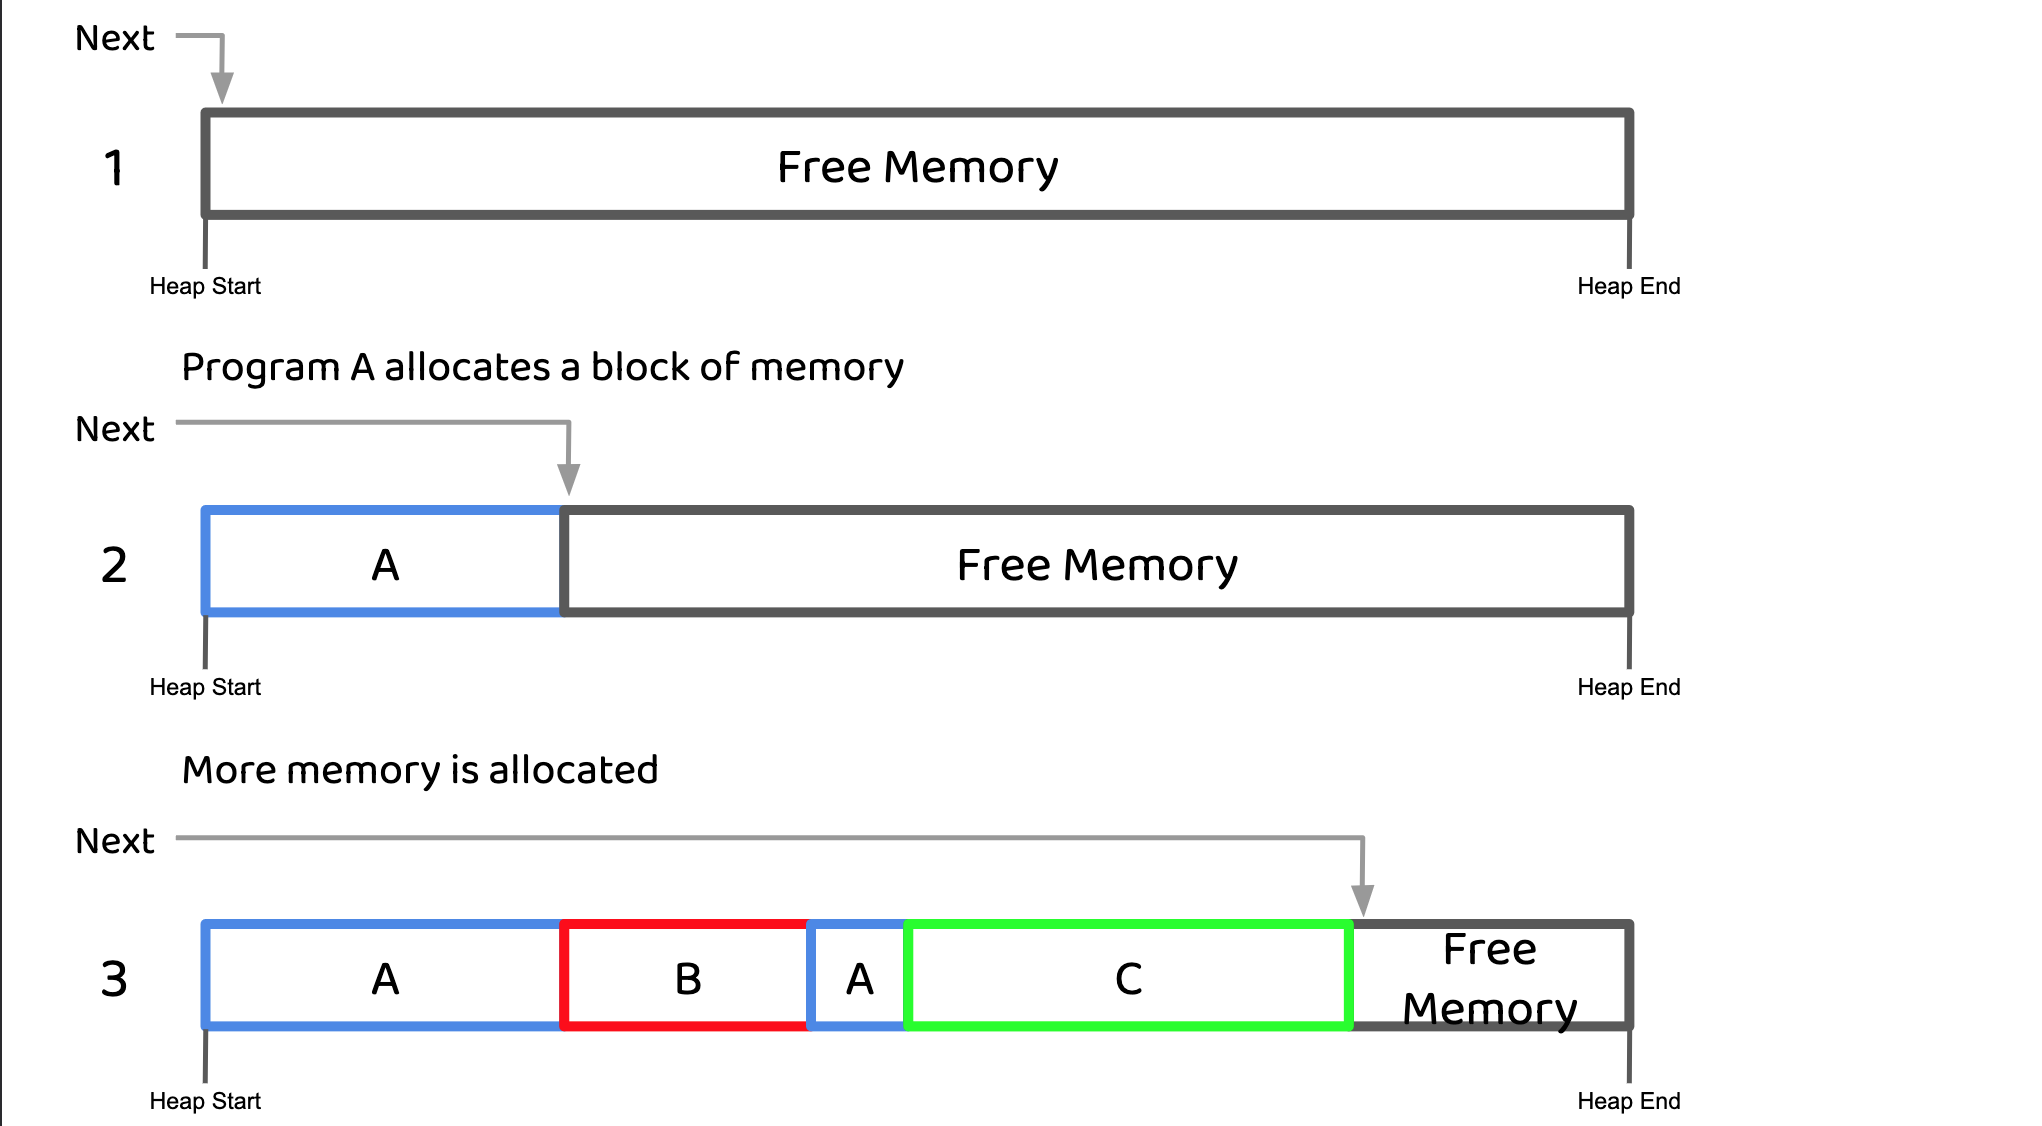
\includegraphics[width=1\textwidth]{mem1.png}
      \caption{Bump Allocation}
      \label{fig:mem1}
\end{figure}

Memory can also be deallocated just by freeing that chunk of memory without changing the \var{next} pointer as see 
in Figure \ref{fig:mem2}.

\begin{figure}[H]
      \centering
      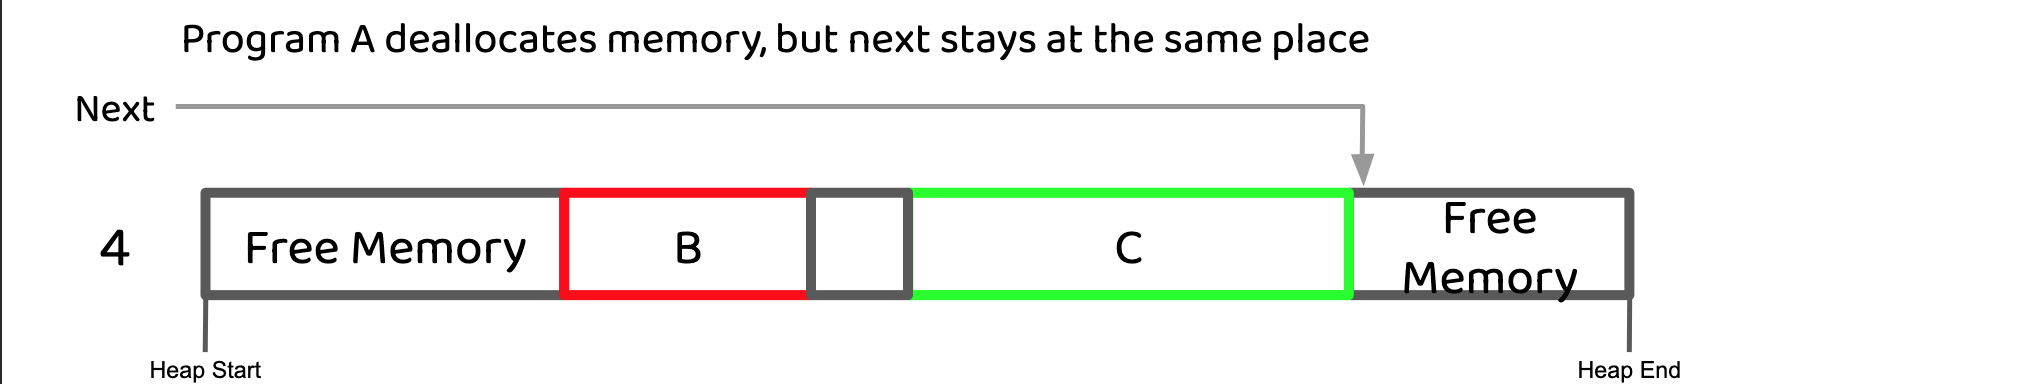
\includegraphics[width=1\textwidth]{mem2.png}
      \caption{Bump deallocation}
      \label{fig:mem2}
\end{figure}

However, there are limitations to this approach. Since the \var{next} pointer only moves forward, it cannot reuse memory 
that has been deallocated. This means that when the allocator reaches the end of the available memory in the heap, 
it runs out of space to allocate any more memory as seen in Figure \ref{fig:mem3}. As a result, the following 
allocation request will result in an out-of-memory error. This approach can also lead to fragmentation that can 
make this memory allocation algorithm less efficient.

\begin{figure}[H]
      \centering
      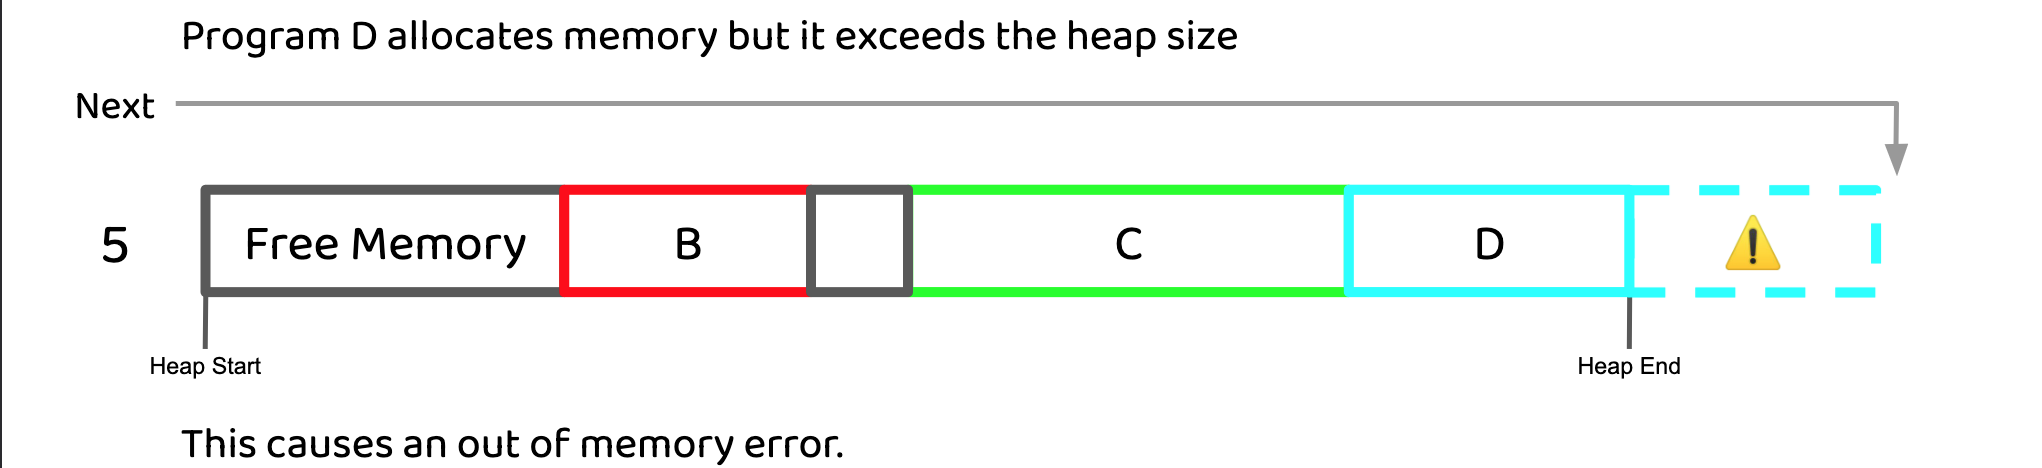
\includegraphics[width=1\textwidth]{mem3.png}
      \caption{Out Of Memory Error}
      \label{fig:mem3}
\end{figure}

To mitigate this issue, an allocation counter can be implemented. This counter increases by one when memory is 
allocated and decreases by one when memory is deallocated. This allows the bump allocator to reset back to the 
beginning of the available memory when the counter reaches zero. However, there is still a possibility of 
encountering an out-of-memory error if the allocation counter is greater than one when it reaches the end of the 
available memory.

\medskip

To fix some of these problems I used a Linked List Allocator Instead.

\subsection{Linked List Allocator:}

A simple linked list allocator is similar to a bump allocator. It uses a linked list, which is a chain of nodes, to 
allocate and deallocate memory as needed.

Initially, the entire memory block is treated as a single free block, as seen in Figure \ref{fig:mem4}, and a linked list node 
is created to represent it. This node contains information regarding the block's size and a reference that points 
to the next node in the list.

\begin{figure}[H]
      \centering
      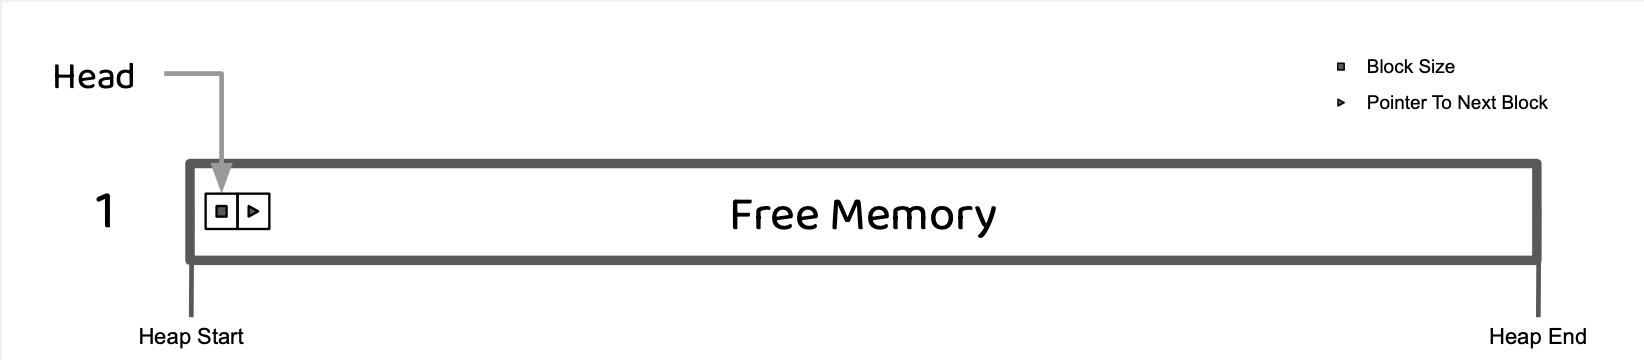
\includegraphics[width=1\textwidth]{mem4.png}
      \caption{Empty Linked List}
      \label{fig:mem4}
\end{figure}

Upon receiving a memory allocation request, the allocator traverses the linked list, starting at the head node and 
following the references to the other nodes, to locate a suitable free block that can accommodate the requested size. 
Once found, the allocator divides the free block into two segments: one for the allocated memory and another for the 
remaining unused memory. The allocated block is marked as "in-use," while the unused block is transformed into a new 
free block by updating it with its own linked list node.

\begin{figure}[H]
      \centering
      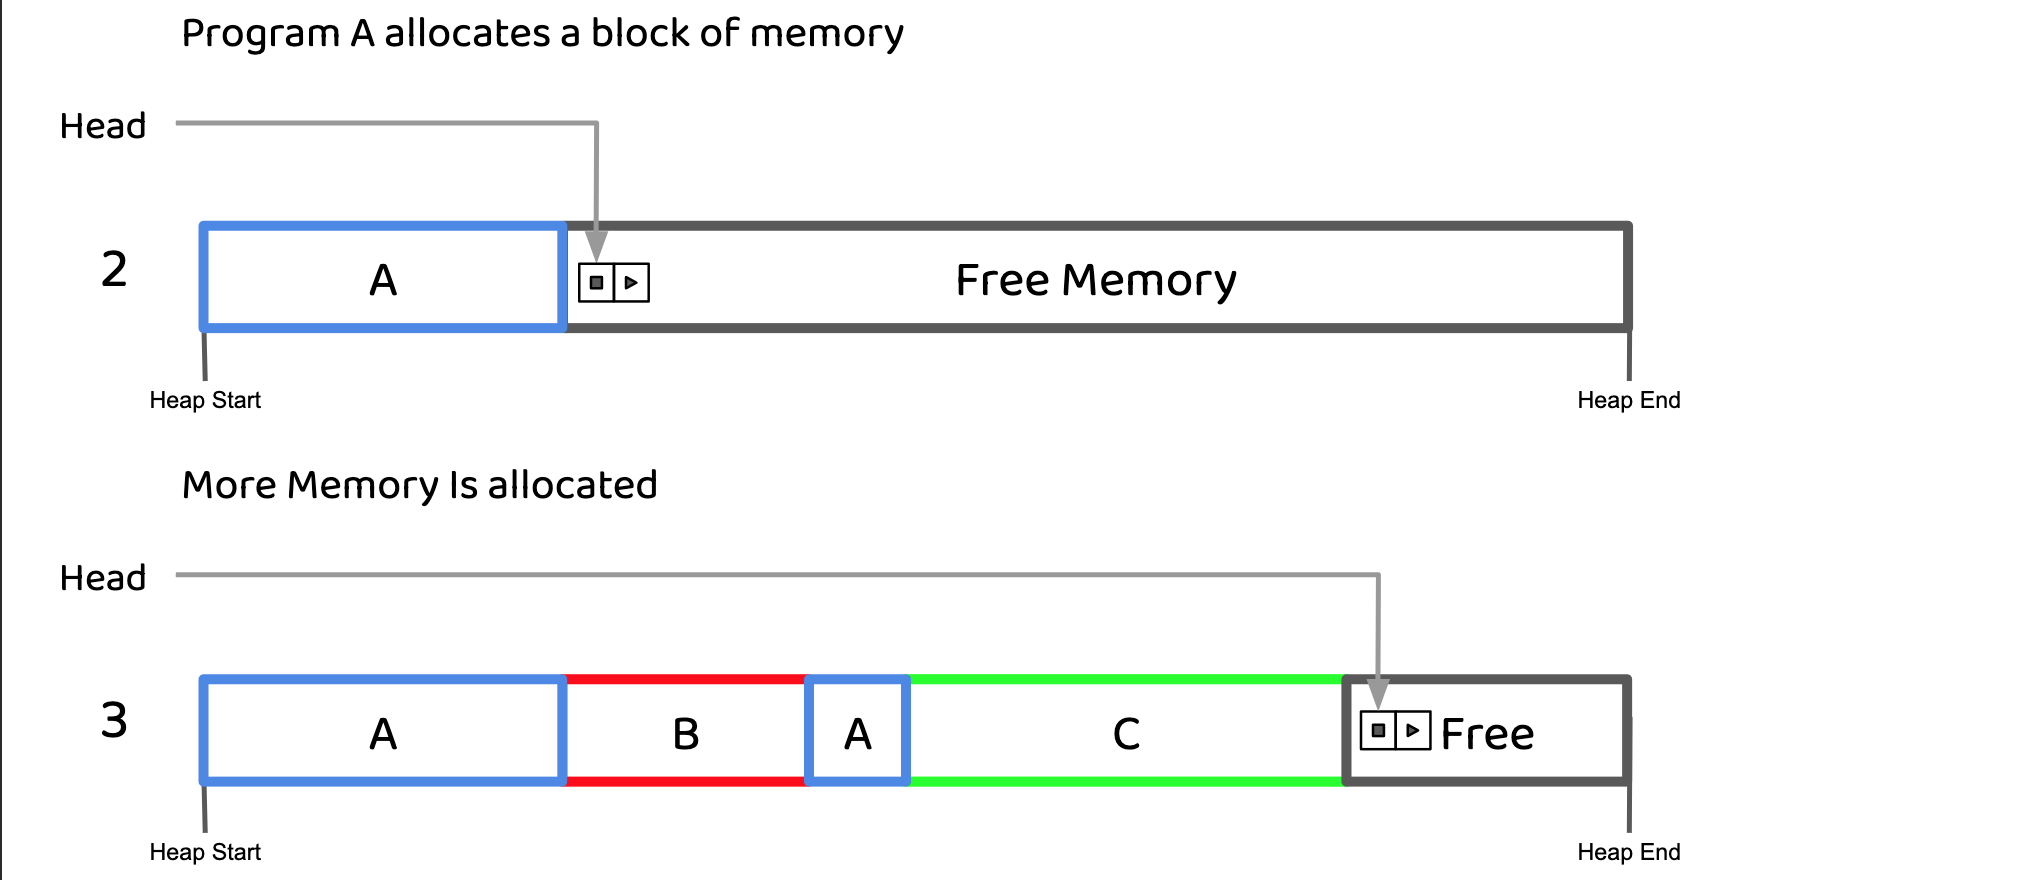
\includegraphics[width=1\textwidth]{mem5.png}
      \caption{Linked List Allocation}
      \label{fig:mem5}
\end{figure}

When memory is no longer needed and is deallocated, the allocator marks that block as free again. It then creates 
a new node that the head points towards. Then, the new node points to the previous node the head was pointing 
towards to complete the list as shown below: 

\begin{figure}[H]
      \centering
      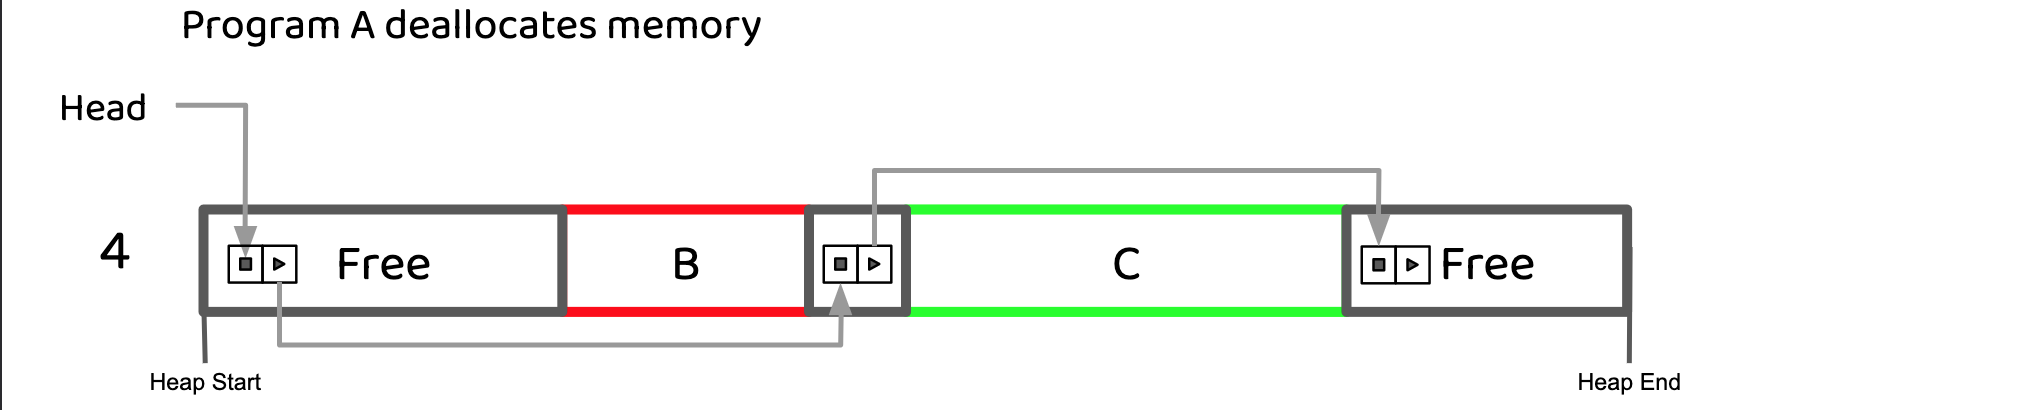
\includegraphics[width=1\textwidth]{mem6.png}
      \caption{Linked List Allocation}
      \label{fig:mem6}
\end{figure}

While a linked list allocator offers flexibility in managing memory allocation and deallocation, it may encounter 
fragmentation issues over time if memory is allocated and deallocated irregularly, leading to a fragmented linked 
list of free blocks like shown:

\begin{figure}[H]
      \centering
      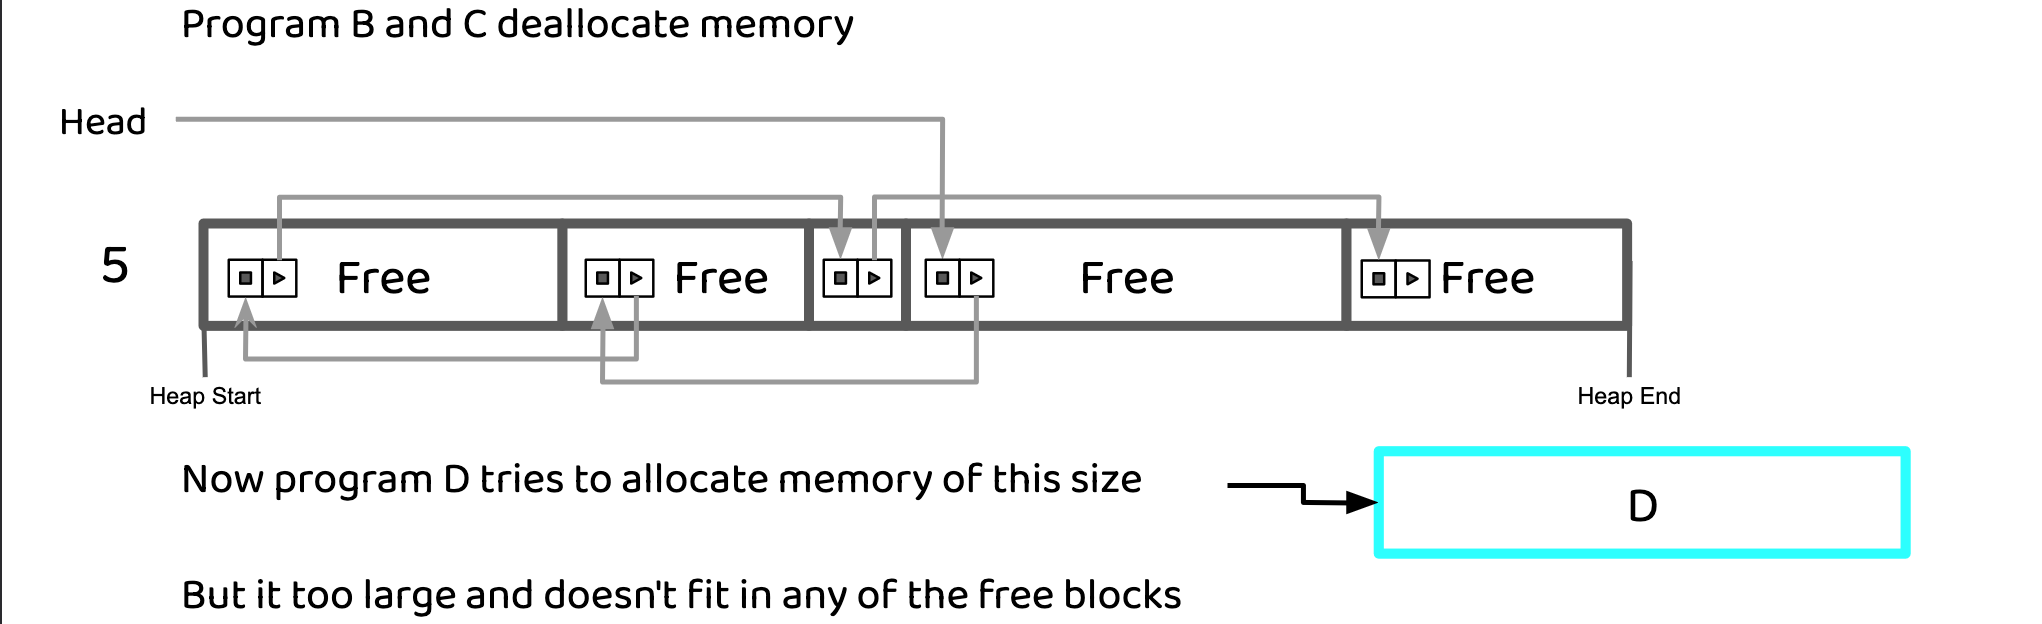
\includegraphics[width=1\textwidth]{mem7.png}
      \caption{Fragmentation In Linked Lists}
      \label{fig:mem7}
\end{figure}

If the linked list is fragmented, whenever a program tries to allocate a single block of memory larger than any of 
the fragmented blocks, it results in an out of memory error because it cannot allocate any memory.

To fix this issue, a compactor can be implemented. The compactor is responsible for rearranging the linked list of 
free memory blocks by consolidating consecutive blocks into larger contiguous blocks. This helps to reduce 
fragmentation and maximize the utilization of available memory. By compacting the blocks, the allocator can ensure 
that larger chunks of continuous memory are available for allocation, improving overall efficiency.

\begin{figure}[H]
      \centering
      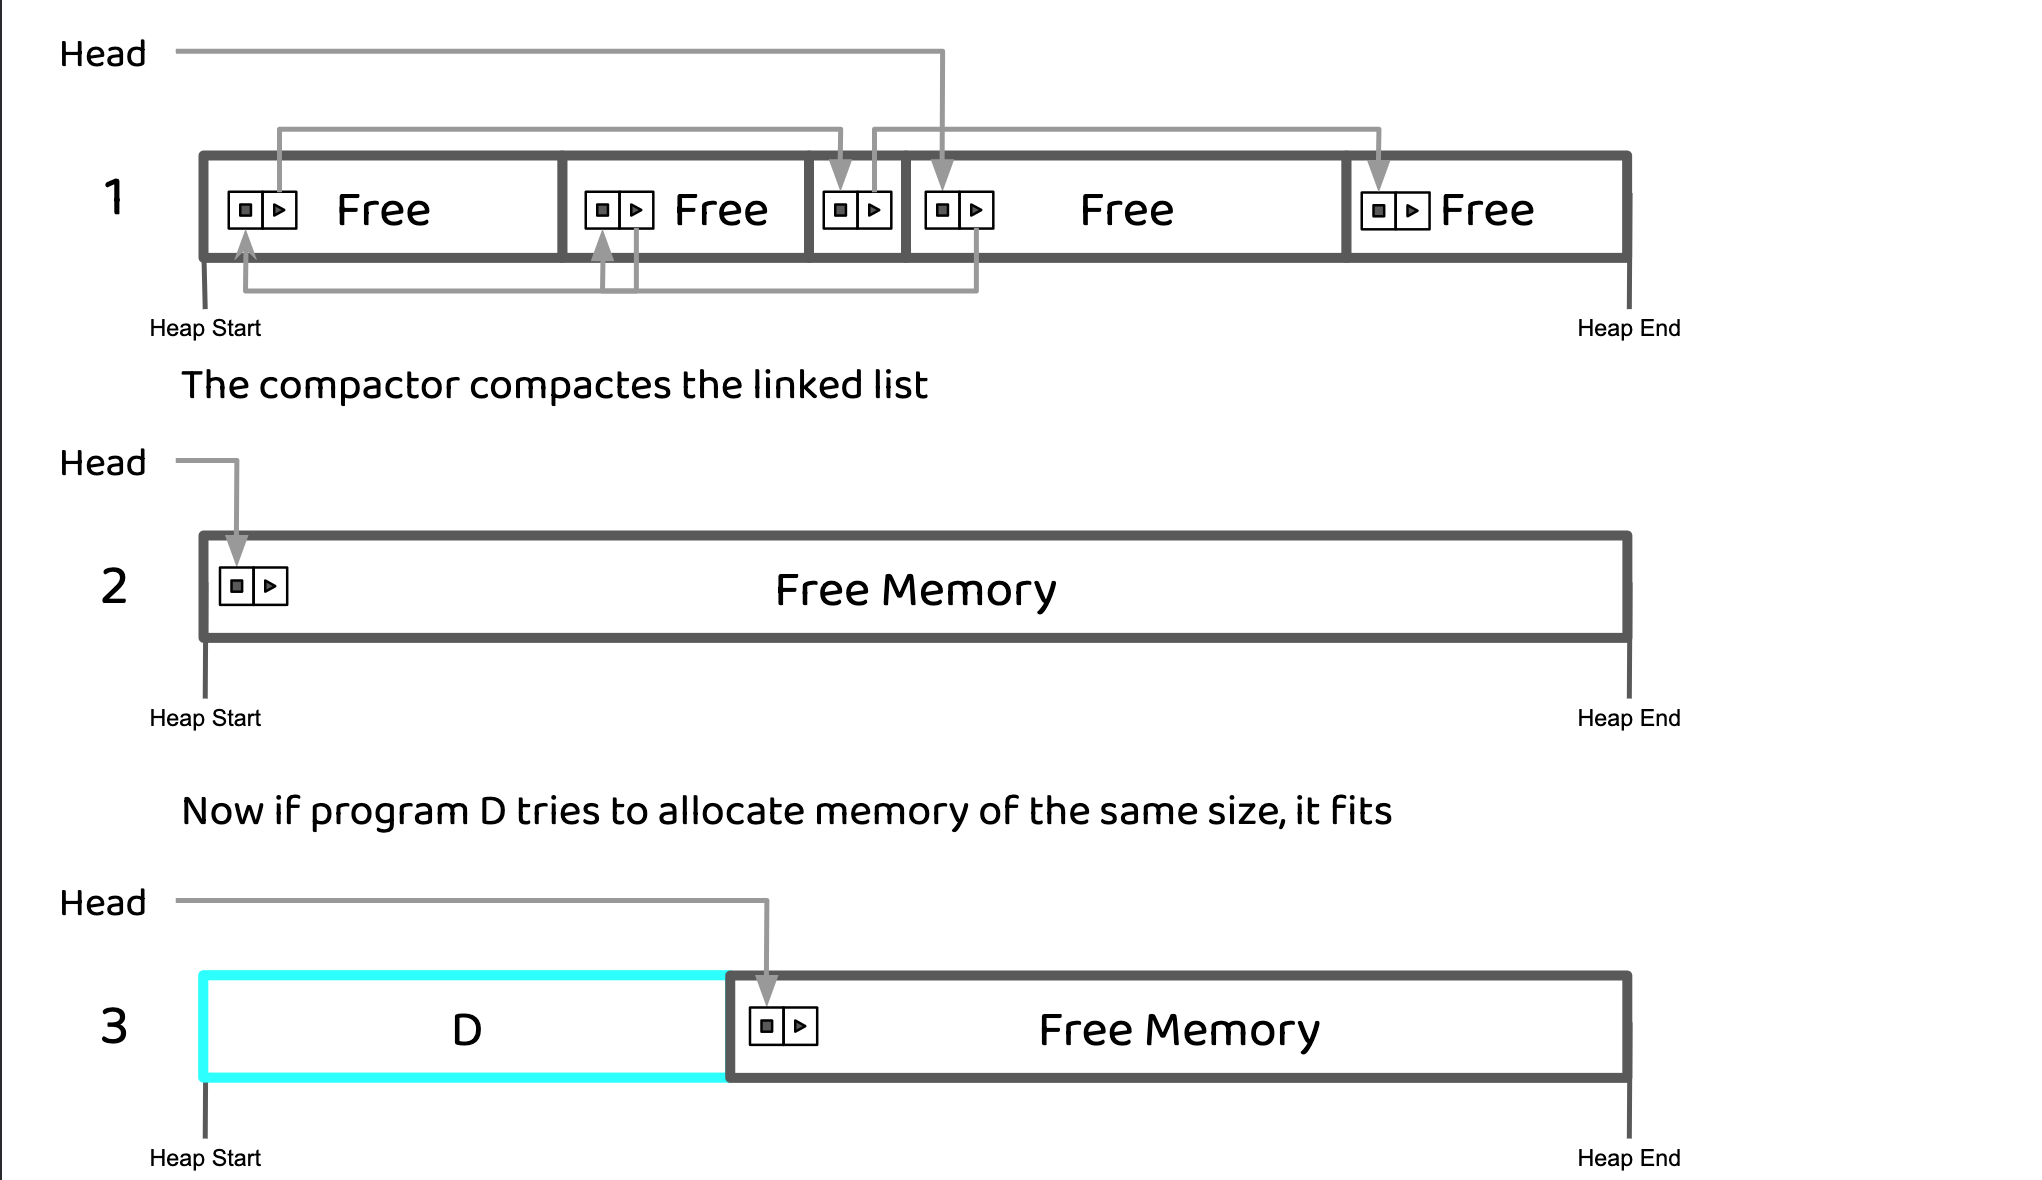
\includegraphics[width=1\textwidth]{mem8.png}
      \caption{Linked List Compaction}
      \label{fig:mem8}
\end{figure}

Unfortunately this is a complicated algorithm to implement, so my linked list currently cannot do this. But it is 
something I would like to implement in the future.

A a simple linked list allocator provides a fundamental yet effective approach to dynamically manage memory 
allocation. It strikes a balance between simplicity and memory utilization efficiency, enabling variable-sized 
memory requests to be handled proficiently.


\section{Current Limitations of My Kernel}

My kernel has many limitations that I will improve on in the future, the most prominent being:
\begin{itemize}
\item Cannot compile programs
\item Fragmentable heap management
\item Lack of features
\end{itemize}

\section{My Expert}

My brother, Jack Maloney, who is a skilled software engineer, played a crucial role in this project. He helped me find 
and fix problems, add new features, and understand complex concepts about computer architecture. I am really grateful 
that he was there to support me throughout the project, and his contributions were a major factor in its success.

\printbibliography

\end{document}